\documentclass[PI,KR]{HSEUniversity}
% Возможные опции: KR или VKR; PI или BI

%%% Работа с таблицами
\usepackage{array,tabularx,tabulary,booktabs} % Дополнительная работа с таблицами
\usepackage{longtable}  % Длинные таблицы
\usepackage{multirow} % Слияние строк в таблице

\title{Разработка Информационной системы для поиска исполнителей по техническому заданию прикладного проекта}
\author{Соломатин Роман Игоревич}
\supervisor{к.т.н., доцент кафедры Информационных технологий в бизнесе НИУ ВШЭ-Пермь}{А. В. Бузмаков}
\Year{2021}
\Abstract{
	Ежедневно появляется множество тендеров, в которых можно принять учатие. Но на подготовку к нему отводистся мало времени. Данная работа посвящена проблеме поиска исполнителей по текстовому описанию задачи.
	
	Количество страниц – 25, количество иллюстраций – 7, количество таблиц –3. $$TO \ DO$$
}

% Ссылка на файл с описание библиографии
\bibliography{library.bib}

\begin{document}

% Обязательные элементы оформления: заголовочный слайд, аннотация, оглавление
\maketitle

\chapter*{Введение}

Каждый день выкладывается несколько десятков тендеров, сроки участия в которых очень сжаты, и потенциальным исполнителям надо быстро определиться смогут они выполнить проект или нет. Для принятия надо ознакомиться с проектом, собрать команду профессионалов для участия и подготовить заявку. Это все очень сложно успеть за месяц. В <<Высшей школе экономики>> много людей с разными компетенциями, и надо по текстовому описанию задачи понять, кто его сможет сделать. Для этого нужно определить, в чем каждый из работников университета компетентен. 

В рамках ВШЭ преподаватели пишут в основном 2 вида научных работ -- статьи в научные журналы и выпускные курсовые работы, которые пишут студенты под их руководством. Анализируя эти тексты можно выделить сферы интересов преподавателей. Для этого были выбраны ВКР, потому что для доступа ко многим научным журналам требуется платная подписка и все работы находятся на многих разных сайтах, с которыми не удобно работать, также статьи часто пишутся на разных языках, что тоже затрудняет работу. А выпускные курсовые работы похожи на статьи, находятся в свободном доступе и содержат много текста для получения компетенций. Таким образом, можно получить сферу компетенций преподавателя, по которой в дальнейшем искать соответствие между пришедшем текстовым описанием задачи и профилем преподавателя. Получается, есть проблемы поиска исполнителей на проект. 

В этой работе будет проверятся гипотеза можно ли из выпускных курсовых работ студентов получить сферу компетенций преподавателя по которой в дальнейшем искать соответствие с текстовым описанием задачи.

Объект исследования - процесс поиска исполнителей по текстовому описанию задачи.

Предмет исследования - автоматизация процесса из объекта.

Цель работы – создать информационную систему для поиска исполнителя по текстовому описанию задачи.

Для достижения поставленной цели нужно сделать:

В первой главе постановка задачи.

Во второй главе описание проектирования системы.

В третьей главе пример работы приложения.

Работа оформлена в соответствии с правилами написания курсовых работ \cite{HSEDocuments}.
\chapter{Анализ предметной сферы}
\section{Обзор существующих решений}
Не существует программных продуктов, которые решают данную задачу в явном виде. Потому что это очень особенная ситуация, когда есть много исполнителей с разными компетенциями и надо для них подбирать задания. Также редко в каких организациях по текстам, которые пишут исполнители можно представить их компетенции. Сейчас это проблема решается вручную.

Приходит в ВШЭ много технических заданий, из отбирает человек, который знает компетенции многих исполнителей. После этого если он думает, что компетенции исполнителя подходят для проекта, то пишет ему. Сотрудник отвечает готов или не готов. Потом за короткий промежуток времени (обычно месяц) нужно подготовить заявку на проект, задать уточняющие вопросы организатору, найти недостающих исполнителей. Данный процесс занимает много времени. Эта система имеет недостатки:
\begin{itemize}
	\item Много проектов теряется, так как человек не знает все компетенции всех исполнителей
	\item Сложно искать проекты
	\item Тяжело масштабировать, потому что необходимо знать много про разных людей
	\item Тратится много времени
\end{itemize}

Иногда применятся способ массовой рассылки требующихся исполнителей для проекта. У данного подхода недостатки: 
\begin{itemize}
	\item Массовую рассылку не все читают
	\item Не дает полную информацию
\end{itemize}

Разрабатываемая система поможет автоматизировать процессы:
\begin{itemize}
	\item Определения компетенций сотрудника
	\item Поиск сотрудников для выполнения задания
\end{itemize}
\begin{FIGURE}[h]{Автоматизация бизнес-процесса "Подбор исполнителя для проекта" \label{fig:figure1}}
	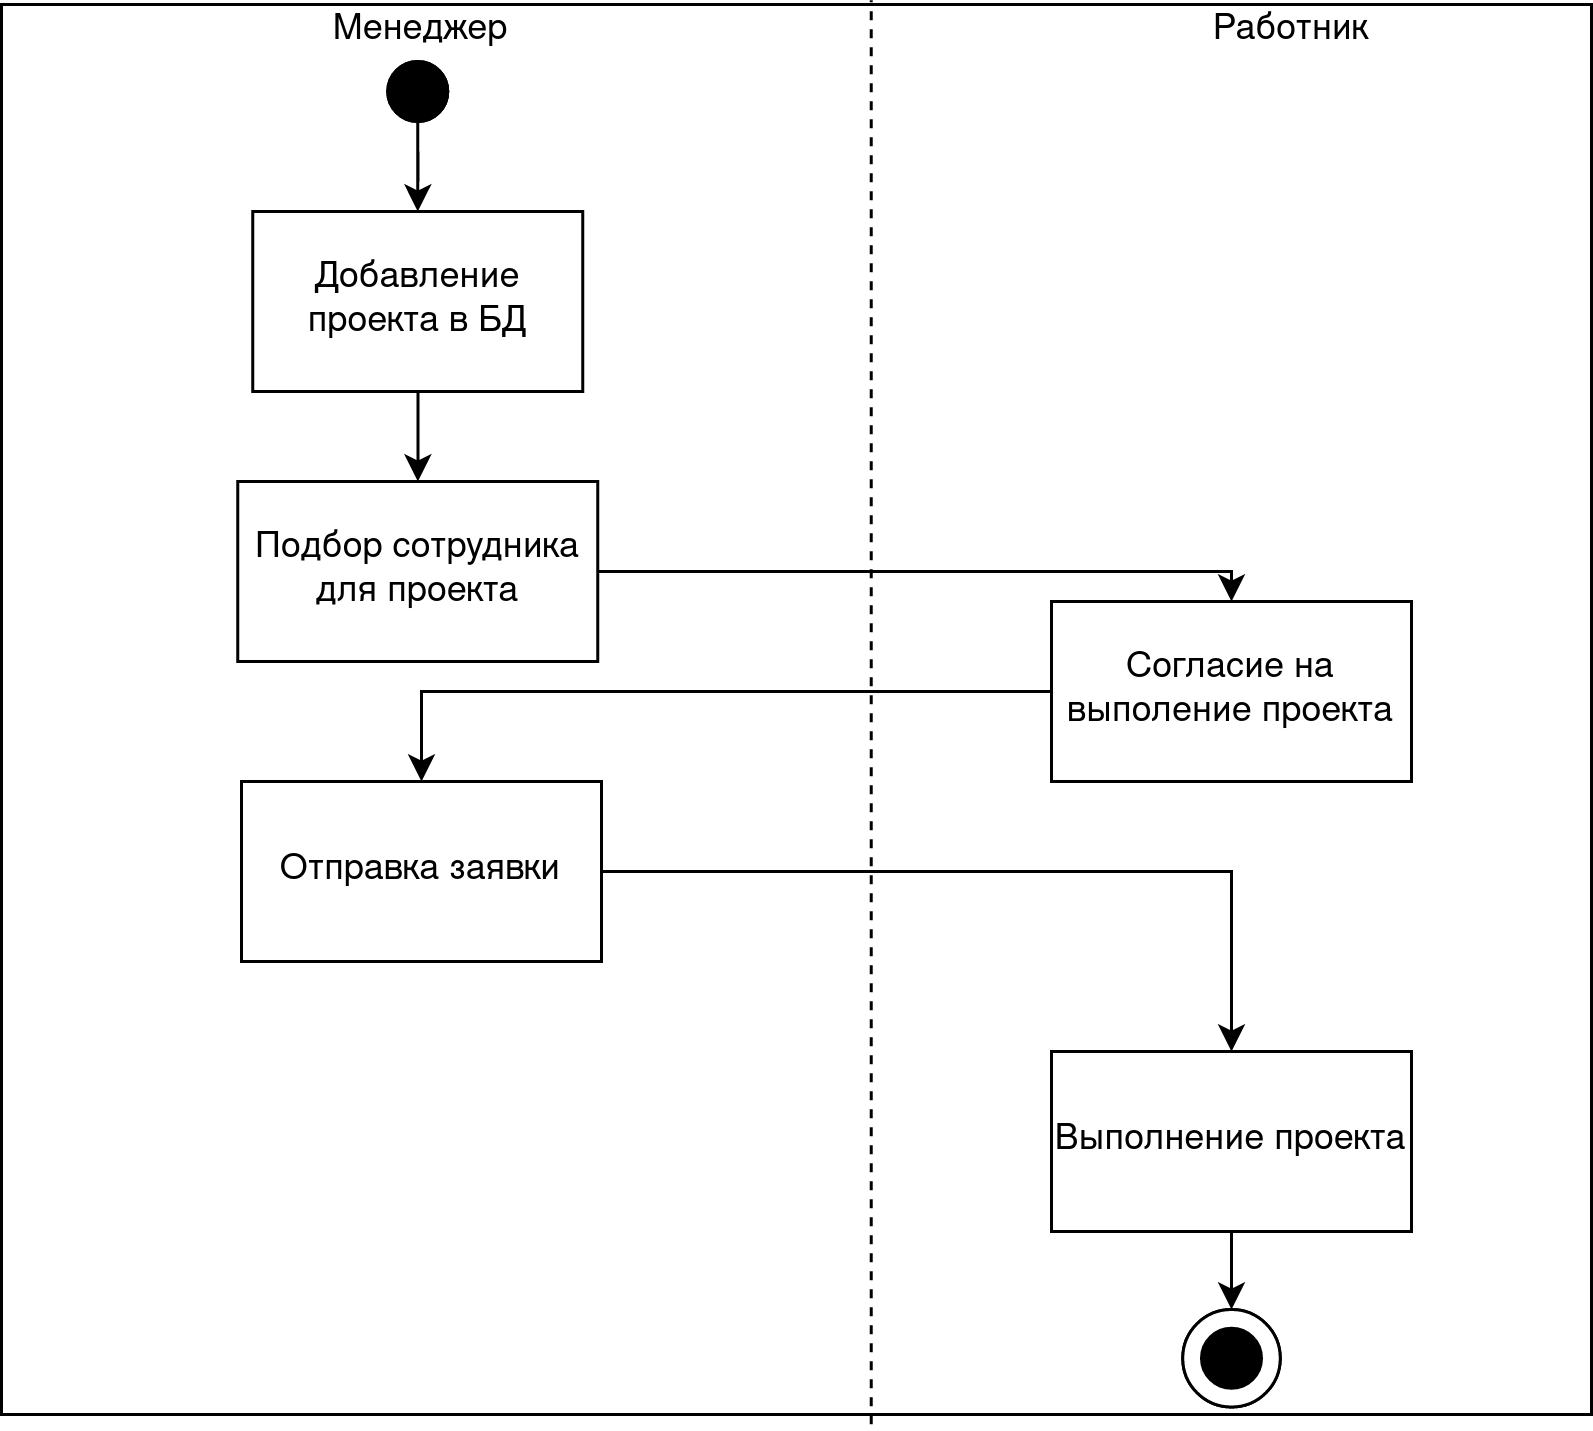
\includegraphics[width=0.6\textwidth]{img/Диаграмма Бизнес-процесса 1}
\end{FIGURE}
Варианты использования реализуемой системы:
\begin{itemize}
	\item Просмотр активных проектов
	\item Поиск компетенций исполнителя
	\item Подбор сотрудника для проекта
	\item Редактирование информации о исполнителя
\end{itemize}

Так как в данной работе нужно проверить гипотезу, будет разрабатываться прототип программы. Диаграмма вариантов использования конечного программного продукта \ref{fig:figure2}.
\begin{FIGURE}[h]{Диаграмма вариантов использования \label{fig:figure2}}
	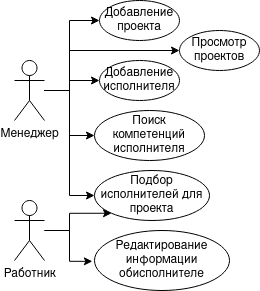
\includegraphics[width=0.6\textwidth]{img/Диаграмма вариантов использования}
\end{FIGURE}

\subsection{Описание прецедента <<Добавление проекта>>}
Предоставляется текстовое описание проекта и потом для него подбираются исполнители из базы данных.
\subsection{Описание прецедента <<Просмотр проектов>>}
Выдаётся список проектов, на которые были отправлены заявки об участии в проекте.
\subsection{Описание прецедента <<Добавление исполнителя>>}
Добавление исполнителя в базу данных, и запись данных о нем.
\subsection{Описание прецедента <<Поиск компетенций исполнителя>>}
Создание компетенций для заданного человека. Для этого надо обработать тексты ВКР с его профиля на сайте <<Высшей школы экономики>>, которые хранятся в формате docx, doc или pdf. \ref{fig:Find actor}
\begin{FIGURE}[h]{Поиск компетенций исполнителя \label{fig:Find actor}}
	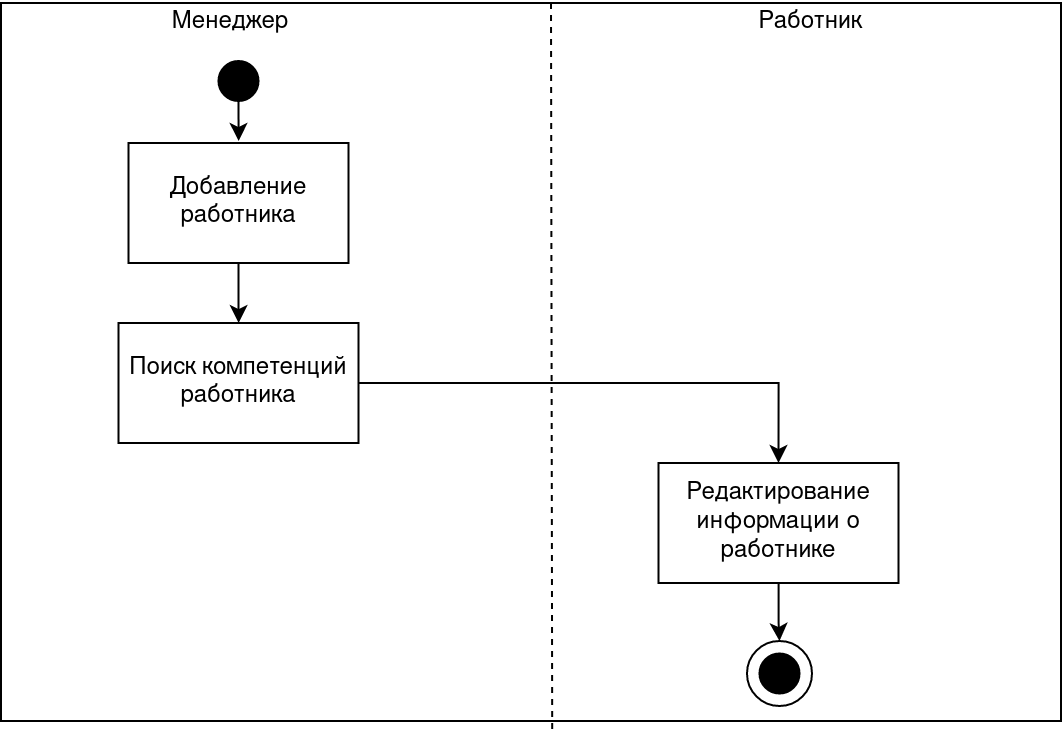
\includegraphics[width=0.6\textwidth]{img/Диаграмма Бизнес-процесса 2}
\end{FIGURE}
\subsection{Описание прецедента <<Подбор исполнителя для проекта>>}
Подбор исполнителя под текстовое описание проекта. \ref{fig:figure1}
\subsection{Описание прецедента <<Редактирование информации об исполнителе>>}
Редактирование данных исполнителя.
\subsection{Описание прототипа}
Основной целью данной работы является проверка гипотезы. Поэтому будет разрабатываться прототип, который будет включать в себя только следующие функции:
\begin{FIGURE}[h]{Диаграмма вариантов использования \label{fig:figure3}}
	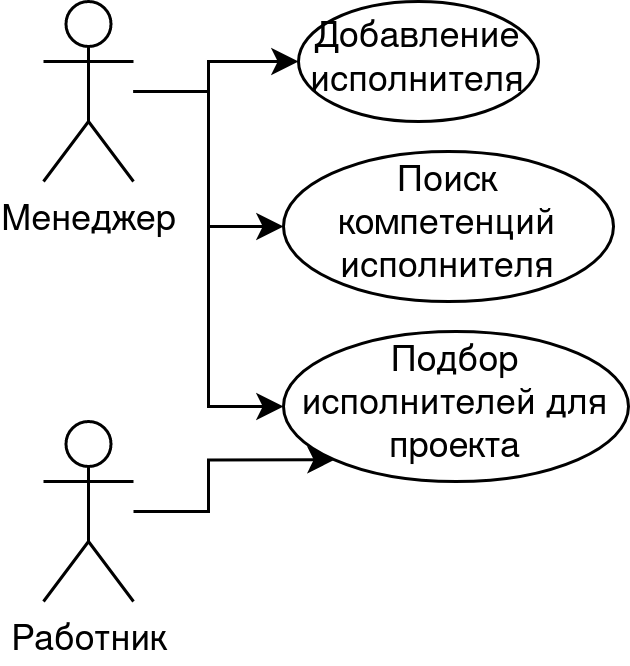
\includegraphics[width=0.6\textwidth]{img/Диаграмма вариантов использования прототипа}
\end{FIGURE}
\begin{itemize}
	\item Добавление исполнителей
	\item Поиск компетенций исполнителей
\end{itemize}
\section{Выбор языка программирования}
Для прототипирования подходят многие языки программирования, вот некоторые из них: Python, C\#, Java, JavaScript. Определимся с основными критериями для выбора языка:

\begin{itemize}
	\item Библиотеки для обучения моделей. Для работы с моделями машинного обучения.
	\item Предобученные модели. Так как для обучения модели надо иметь большой объем данных и много вычислительных мощностей.
	\item Библиотеки для обработки сайта.
	\item Библиотека для обработки docx и pdf файлов и обработки сайтов.
	\item Интерактивный режим. Позволяет просмотреть данные, преобразовать их, вмешаться в исполнение кода. Выполнить в произвольном порядке.
\end{itemize} 

\begin{TABLE}[!h]{Таблица сравнения языков программирования \label{tbl:tableProg}}
	\begin{tabular}[c]{|p{3cm}|p{2cm}|p{3cm}|p{2cm}|p{2cm}|p{3cm}|}
		\hline
		Язык программирования & Библиотека для МО & Предобученные модели & Работа с сайтом & Работа с файлами & Интерактивный режим\\ \hline
		Python 		& ++ & ++ & + & + & + \\ \hline
		C\# 		& +  & +  & + & + & - \\ \hline
		Java 		& +  & +  & + & + & - \\ \hline
		JavaScript 	& +  & +  & + & + & ? \\ \hline
	\end{tabular}
\end{TABLE}

Под эти критерии подходит Python. Он простой для написание и отладки, так как это интерпретируемый язык программирования, у него есть интерактивный режим. Также есть фреймворк PyThorch и библиотека с предобученными моделями HuggingFace Transformers, в частности RuBERT \cite{kuratov2019adaptation}, а также есть библиотека Bert Extractive Summarizer \cite{miller2019leveraging} для удобной работы с моделей.

\section{Выбор СУБД}
Для Python существуют библиотеки для работы с любыми системами управления базами данных. Для курсовой работы был выбран SQLite потому что его легко настраивать, нет необходимости устанавливать ничего дополнительно, что достаточно для прототипирования с небольшим количеством данных. 300 преподавателей и 1700 выпускных квалификационных работ.
\chapter{Проектирование системы}
\section{Проектирование базы данных}
Для разработки системы необходимо хранить информации о преподавателях и выпускных квалификационных работах, где они были руководителями была разработана база данных. Необходимо было хранить:

\begin{description}
	\item [Код преподавателя] -- уникальный код преподавателя для его идентификации в базе данных
	\item [ФИО преподавателя] -- фамилия имя и отчество преподавателя
	\item [Ссылка на профиль преподавателя] -- ссылка на профиль преподавателя на сайте Высшей школы экономики, для последующей проверки в ручную при подборе на проект
	\item [Код статуса] -- код статуса для последующей связи в базе данных
	\item [Код кафедры] -- код кафедры для последующей связи в базе данных
	\item [Компетенции] -- компетенции преподавателя полученные путём автоматического анализа текстов ВКР в текстовом виде
	\item [Эмбеддинги] -- компетенции преподавателя полученные путём автоматического анализа текстов ВКР в векторном пространстве для дальнейшего подбора исполнителя для проекта
	
	\item [Код статуса] -- уникальный код статуса для идентификации в базе данных
	\item [Наименования статуса] -- доцент, старший научный сотрудник и тд. Для представление информации о преподавателе.
	
	\item [Код кафедры] -- уникальный код кафедры для идентификации в базе данных
	\item [Наименование кафедры] -- название кафедры, где работает преподаватель. Для представление информации о преподавателе.
	
	\item [Код кампуса] -- уникальный код для идентификации в базе данных
	\item [Наименования кампуса] -- название кампуса. Для представление информации о преподавателе.
	
	\item [Код ВКР]  -- уникальный код выпускной квалификационной работы для идентификации в базе данных
	\item [Название ВКР] -- название выпускной квалификационной работы. Необходимо для дальнейшего соотнесения в преподвателя ручном режиме
	\item [Научный руководитель] -- код преподавателя для последующей связи в базе данных
	\item [Ссылка на ВКР] -- ссылка на выпускную квалификационную работу на сайте ВШЭ для проверки корректности сбора информации
	\item [Ссылка на полный текст ВКР] -- ссылка на файл для загрузки с полным текстом ВКР
	\item [ФИО студента] -- фамилия имя и отчество студента написавшего ВКР
	\item [Код ОП студента] -- код образовательной программы студента для последующей связи в базе данных
	\item [Код кампуса] -- код кампуса для последующей связи в базе данных
	
	\item [Код образовательной программы] -- уникальный код для идентификации в базе данных
	\item [Код факультета] -- код факультета для последующей связи в базе данных
	\item [Наименование ОП] -- название образовательной программы, где обучается студент
	
	\item [Код факультета] -- уникальный код факультета для идентификации в базе данных
	\item [Наименование факультета] -- название факультета
\end{description} 
Описание данных для проектирования БД \ref{tbl:tableDB}.
\begin{TABLE}[!h]{Таблица атрибутов \label{tbl:tableDB}}
	\begin{tabular}[c]{|p{4cm}|l|p{3cm}|l|p{3cm}|}
		\hline
		Имя атрибута & Тип данных & Значение по умолчанию & Формат ввода & Ограничение на значения\\ \hline

		Код преподавателя 				& Число  & Нет & Нет 		& Нет \\ \hline
		ФИО преподавателя 				& Строка & Нет & Нет 		& Нет \\ \hline	
		Ссылка на профиль преподавателя & Строка & Нет & Нет 		& Нет \\ \hline
		Компетенции 					& Строка & Нет & Нет 		& Нет \\ \hline
		Эмбеддинги 						& Число  & Нет & Нет 		& Нет \\ \hline
		Код ВКР 						& Число  & Нет & Нет 		& Нет \\ \hline
		Название ВКР 					& Строка & Нет & Нет 		& Нет \\ \hline
		Ссылка на ВКР 					& Строка & Нет & Нет 		& Нет \\ \hline
		Ссылка на полный текст ВКР 		& Строка & Нет & Нет 		& Нет \\ \hline
		ФИО студента 					& Строка & Нет & Нет 		& Нет \\ \hline
		Код ОП студента 				& Число  & Нет & 00.00.00	& Нет \\ \hline
		Код статуса 					& Число  & Нет & Нет		& Нет \\ \hline
		Наименования статуса 			& Строка & Нет & Нет 		& Нет \\ \hline
		Код кафедры 					& Число  & Нет & Нет 		& Нет \\ \hline
		Наименование кафедры 			& Строка & Нет & Нет 		& Нет \\ \hline
		Код кампуса 					& Число  & Нет & Нет 		& Нет \\ \hline
		Наименования кампуса 			& Строка & Нет & Нет 		& Нет \\ \hline
		Код образовательной программы 	& Число  & Нет & 00.00.00 	& Нет \\ \hline
		Код факультета		 			& Число  & Нет & Нет 		& Нет \\ \hline
		Наименование ОП 				& Строка & Нет & Нет	 	& Нет \\ \hline
		Код факультета 					& Число  & Нет & Нет 		& Нет \\ \hline
		Наименование факультета 		& Строка & Нет & Нет 		& Нет \\ \hline
	\end{tabular}
\end{TABLE}
\subsection{Приведение к 1НФ}
Данные находятся в первой нормальной форме, если атрибуты атомарны и неделимы, состоят из элементарных составляющих и отсутствуют дубликаты.
\begin{enumerate}
	\item \underline{Код преподавателя}
	\item ФИО преподавателя
	\item Ссылка на профиль преподавателя
	\item Компетенции
	\item Эмбеддинги
	\item Код статуса преподавателя
	\item Код кафедры преподавателя
		
	\item \underline{Код ВКР}
	\item Название ВКР
	\item Код преподавателя
	\item Ссылка на ВКР
	\item Ссылка на полный текст ВКР
	\item ФИО студента
	\item Код кампуса
	\item Код ОП студента
	
	\item \underline{Код статуса}
	\item Наименование статуса
	
	\item \underline{Код кафедры}
	\item Наименование кафедры
	
	\item \underline{Код кампуса}
	\item Наименования кампуса
	
	\item \underline{Код образовательной программы}
	\item Код факультета
	\item Наименование ОП
	
	\item \underline{Код факультета}
	\item Наименование факультета
\end{enumerate} 

Данные атрибуты находятся в 1НФ.
\subsection{Приведение к 2НФ}
Данные находятся во второй нормальной форме, если они в первой нормальной форме и отсутствует частичная функциональная зависимость не ключевых атрибутов от ключа.
В соответствии с описанными выше зависимостями можно сделать вывод, что в описанном отношении имеются следующие частичные зависимости:
\begin{enumerate}
	\item Код преподавателя определяет:
	\begin{itemize}
		\item ФИО преподавателя
		\item Ссылка на профиль преподавателя
		\item Компетенции
		\item Эмбеддинги
		\item Код статуса преподавателя
		\item Код кафедры преподавателя
	\end{itemize}
	\item Код ВКР определяет:
	\begin{itemize}
		\item Название ВКР
		\item Код преподавателя
		\item Ссылка на ВКР
		\item Ссылка на полный текст ВКР
		\item ФИО студента
		\item Код кампуса
		\item Код ОП студента
	\end{itemize}
	\item Код статуса преподавателя определяет:
	\begin{itemize}
		\item Наименование статуса
	\end{itemize}
	\item Код факультета определяет:
	\begin{itemize}
		\item Наименование факультета
	\end{itemize}
	\item Код кампуса определяет:
	\begin{itemize}
		\item Наименование кампуса
	\end{itemize}
	\item Код кафедры определяет:
	\begin{itemize}
		\item Наименование кафедры
	\end{itemize}
	\item Код образовательной программы определяет:
	\begin{itemize}
		\item Название образовательной программы
	\end{itemize}
\end{enumerate}
\section{Сбор данных}
Для работы программы необходимо собрать данные о преподавателях и ВКР, которые у них писались. Для этого надо было обрабатывать информация находящуюся на сайте ВШЭ. Такая обработка возможна с помощью библиотеки BeautifulSoap, который позволяет получать html любого сайта.

В первую очередь надо было получить список преподавателей и ссылки на их страницы. Для этого обрабатывался сайт со списком преподавателей, но там можно получить преподавателей, фамилии которых начинаются на 1 букву. Что бы решить эту проблему с сайты получались ссылки на буквы. А потом с каждой такой ссылки собирался список преподавателей и ссылки на их страницы. Для этого брались все элементы страницы с атрибутом "a"\ и классом "link"\ , в которых значение атрибута "href"\ было "/org/persons/"\ или "/staff/". В базу данных записывались ФИО преподавателя и ссылку на их страницу. 

Далее надо было получить список ВКР для каждого преподавателя. Для этого брались все элементы страницы с атрибутом "a"\ и классом "link"\ , в которых значение атрибута "href"\ было "/edu/vkr/". Итого получилось собрать информацию о 321 преподавателе и 1708 ВКР.

Потом надо было получить информацию о ВКР, но их данные ВКР, в отличие от данных преподавателей, подгружались после загрузки основой страницы. Чтобы решить эту проблему пришлось эмулировать работу браузера с помощью библиотеки Selenium и драйвера Gecko (движок браузера FireFox). Библиотека Selenium не использовалась раньше, так как для ее работы надо больше времени и ресурсов, поэтому данная библиотека использовалась только на данном этапе. Для полной загрузки страницы ставилась задержка в 2 секунды. И бралась информация атрибута "p"\ с классом "vkr-card\_\_item". Также бралась информация о научном руководителе, он искался в базе данных, и потом в базу данных уже записывался Код преподавателя.

Чтобы получить тексты из файлов, они обрабатывались с помощью textract, которая позволяет получить информацию из pdf, doc и docx файлов, и помещались в базу данных.
\section{Создание профиля человека}
Для создание профиля человека рассматривались TFiDF \cite{das2018improved} и суммаризация текста c помощью BERT \cite{devlin2019bert} (Bidirectional Encoder Representations from Transformers). 

Подход TFiDF заключается в том что бы для каждого слова посчитать его отношение числа вхождений некоторого слова к общему числу слов документа (TF) и частоты, с которой некоторое слово встречается в документах коллекции (DF). Частоты в рамках коллекции рассматриваются для того что бы выявить распространённые слова в данных документах и снизить их важность, например "Информационная система", и наоборот найти слова которые находят важную тему, например "Машинное обучение".  Данный подход часто используется для кластеризации текстов. Но данный метод плохо подходит для данной задачи, потому что он не рассматривает контекст используемых слов. Это значит у него проблемы с омонимами и синонимами. Например, в предложениях "Ключ открыл замок" и "Рыцарь штурмовал замок" слова "зАмок" и "замОк" будут считаться как одно и тоже слово, хотя по контексту это разные слова.

BERT -- это нейросетевая языковая модель, которая рассматривает контекст, в котором находится слово и кодирует данное слово в своём векторном пространстве. Для этого модели подаётся на вход предложение, и каждое слово разделяется на отдельную часть предложения (токенизируется). Потом в начало и конец предложения добавляются специальные токены ([CLS], [SEP]), затем все токены предложения приводятся к нормальной форме слова (лемматизируются). Потом каждому слову присваивается вектор (эмбеддинг), которым кодируется слово. Для предложений также строится свой эмбединг. Цель работы данного алгоритма -- предсказывать следующее слово или понять идут предложения рядом или нет. Пример работы алгоритма \ref{fig:BERT sentences}. 

\begin{FIGURE}[h]{Обработка предложения \label{fig:BERT sentences}}
	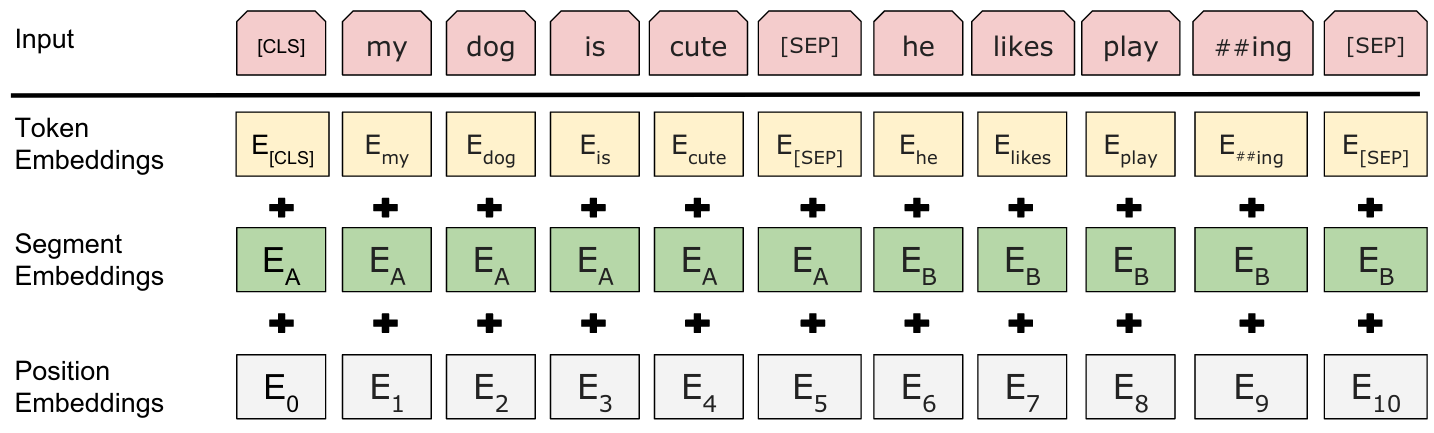
\includegraphics[width=0.6\textwidth]{img/BERT sentences}
\end{FIGURE}

При обучении задачи на предсказание следующего слова нейронная сеть закрывает 15\% слов маской, и пытается предсказывает какие слова были замаскированы на основе контекста. Для этого нейронная сеть находит вектора слов, которые находятся рядом в предложении, и берет близкое слово в векторном пространстве, относительно соседних слов \ref{fig:BERT illustrated}. 

\begin{FIGURE}[h]{Поиск "замаскированного" слова \label{fig:BERT illustrated}}
	\includegraphics[width=0.6\textwidth]{img/BERT illustrated}
\end{FIGURE}

В данной работе использовался предобученный BERT от DeepPavlovAI RuBert \cite{kuratov2019adaptation}, который обучался на русских текстах. 

Для задачи определения последовательности предложений в модель часть предложений поступает в последовательно, а другая часть в случайном порядке. И модель пытается предсказать какие из этих предложений находятся рядом в оригинальном тексте \ref{fig:BERT example}.

\begin{FIGURE}[h]{Схема работы BERT \label{fig:BERT example}}
	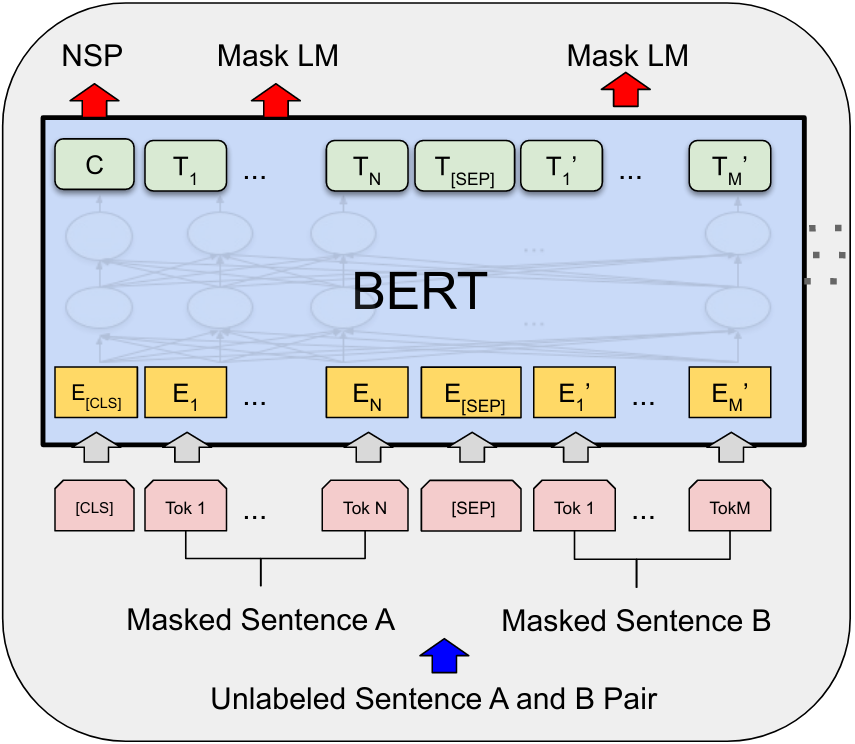
\includegraphics[width=0.6\textwidth]{img/BERT example}
\end{FIGURE}

BERT обрабатывал ВКР, которые написаны у преподавателей. С его помощью мы получили эмбединги предложений из ВКР. Получилось очень много предложений и надо получить короткое описание текстов фиксированного размера для каждого преподавателя. Чтобы сделать это можно взять самые типовые предложения, чем и занимается библиотека BERT Extractive summarizer \cite{miller2019leveraging}. 

BERT Extractive summarizer ищет эмбединги предложений, которые находятся рядом в векторном пространстве и объединяет их в группы (кластеры). И результатом общений текстов будет самое близкое предложение к центру кластера \ref{fig:Summ Knn}, что позволяет получить краткое содержание текста. Таким образом получается описание текста в виде эмбединга, для удобства работы алгоритмически, и текста, для проверки в ручную, остаётся сопоставить описание преподавателя и текстового задания.

\begin{FIGURE}[h]{Пример поиска содержания предложений \label{fig:Summ Knn}}
	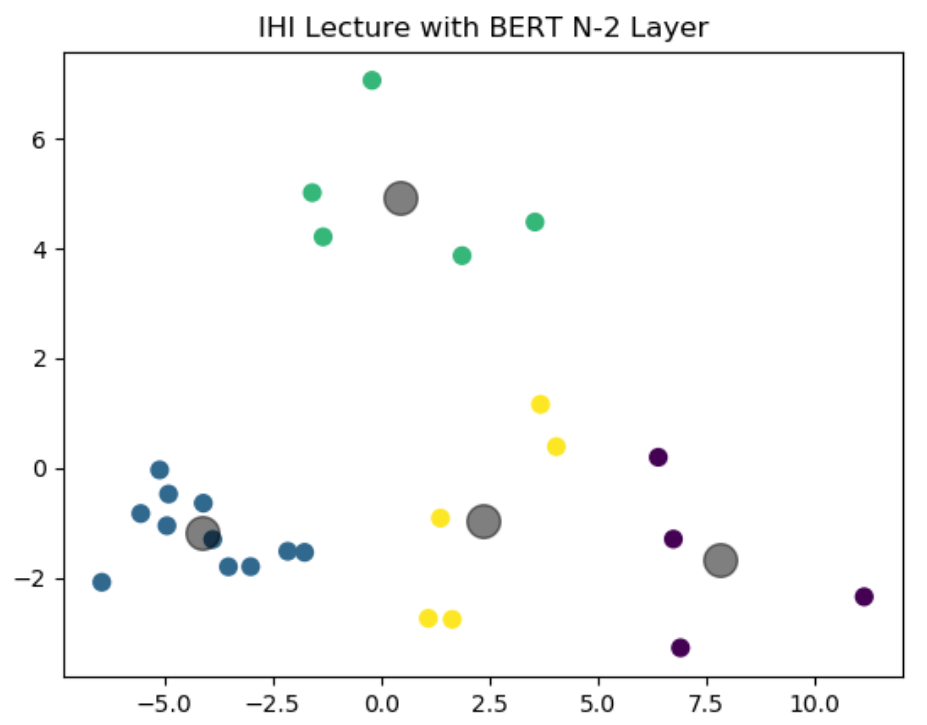
\includegraphics[width=0.6\textwidth]{img/Summ Knn}
\end{FIGURE}

\section{Функции подбора исполнителя}
Для подбора исполнителя сравнивались эмбединнги текстового задания и преподавателя. Для лучшего подбора подходящего человека были разработаны разные функции поиска расстояний. Результатом работы алгоритма является исполнитель с наименьшим расстоянием между описанием задания и компетенциями исполнителя. Реализованные функции расчёта расстояний:
\begin{itemize}
	\item Средняя разница элементов -- в данном методе поиска расстояний, отрицательное расстояние может скомпенсировать положительное.
	\item Модуль разницы элементов (Манхэтонновское расстояние) -- этот метод поиска расстояний будет штрафовать за расстояния, которые находятся близко сильнее, чем расстояние Евклида.
	\item Квадрат разницы элементов  (Евклидово расстояние) --  этот метод поиска расстояний будет штрафовать за расстояния, которые находятся далеко сильнее, чем Манэтонновское расстояние.
\end{itemize}
Нужно было сопоставить 10 эмбедингов текстового описания задания и 10 эмбедингов преподавателя. Для этого было реализовано несколько алгоритмов:
\begin{itemize}
	\item Все со всеми. Каждый эмбединг текста сопоставляется с эмбеднигами преподавателя и считается сумма их расстояний.
	\item Поиск минимального с повторами. Для каждого эмбеддинга текста находится минимальное расстояние с эмбедингом преподавателя и считается сумма каждой такой пары.
	\item Поиск минимального без повторов. Для каждого эмбеддинга текста находится минимальное расстояние с эмбедингом преподавателя, если уже была пара с таким эмбедингом преподавателя, то берётся другой эмбединг с минимальный расстоянием, и считается сумма каждой такой пары.
	\item Усреднение эмбеддингов. Эмбеддинги преподавателя и текста усредняются и считается расстояние между ними.
\end{itemize}
Cхемы подбора находятся в Приложении А.
\chapter{Разработка и тестирование системы}
\section{Разработка интерфейсов}
Для удобства был сделан графический интерфейс\ref{fig:GUI}. С помощью него можно ввести текстовое описание задачи и подобрать походящего исполнителя.
\begin{FIGURE}[h]{Интерфейс приложения \label{fig:GUI}}
	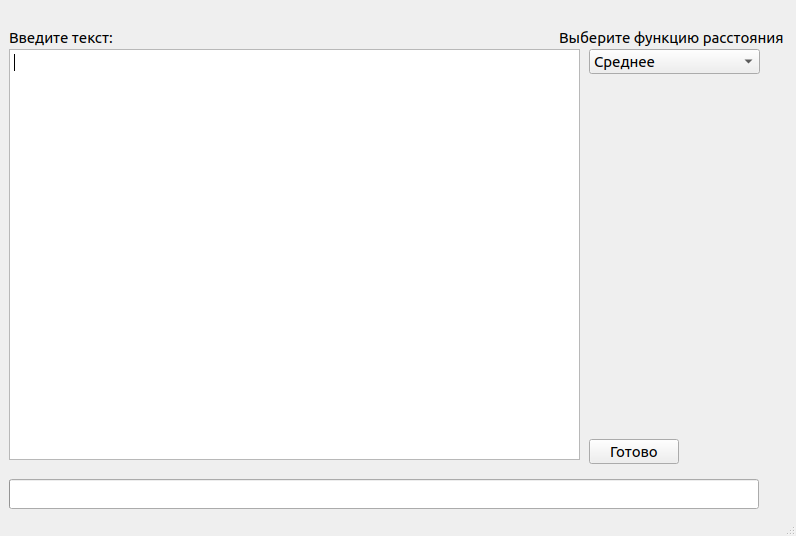
\includegraphics[width=0.6\textwidth]{img/GUI}
\end{FIGURE}

На данном окне есть текстовое поле куда вносится весь текст задания.

Для выбора функции ошибки есть ComboBox, в котором можно выбрать одну из следующих функций ошибки:
\begin{itemize}
	\item Среднее
	\item MAE
	\item MSE
	\item RMSE
\end{itemize}

При нажатии кнопки Готово начинается подбор исполнителя, это занимает в среднем примерно 5 минут, для удобства отслеживания времени работы алгоритма был добавлен ProgressBar в низ приложения.

\section{Тестирование приложения}
Для тестирования приложения была выбрана выпускная квалификационная работа Абросимовой П. С. с темой <<Разработка средств автоматизации расширения онтологии на основе данных интернет-источников>> руководителем была Лядова Л. Н. Для тестирования в коде было сделано так чтобы, данный научный сотрудник не был решением алгоритма. Результаты работы разных алгоритмом и функций расстояния \ref{tbl:tableRes}.

\begin{TABLE}[!h]{Результатов работы программы \label{tbl:tableRes}}
	\begin{tabular}[c]{|p{4cm}|l|p{4cm}|l|}
		\hline
		Тип алгоритма        			& Среднее расстояние & Манхэттоновское расстояние & Расстояние Евклида \\ \hline
		Все со всеми		            & Кычкин А. В.       & Кушев В. О.                & Кушев В. О.        \\ \hline
		Поиск минимального с повторами  & Божья-Воля А. А.   & Кычкин А. В.               & Кычкин А. В.       \\ \hline
		Поиск минимального без повторов & Божья-Воля А. А.   & Божья-Воля А. А.           & Божья-Воля А. А.   \\ \hline
		Усреднение эмбеддингов      	& Кычкин А. В.       & Кузнецов Д. Б.             & Кузнецов Д. Б.     \\ \hline
	\end{tabular}
\end{TABLE}

Получилось 4 преподавателя Кычкин А. В., Кушев В. О., Божья-Воля А. А., Кузнецов Д. Б., из которых 3 преподавателя работают на кафедре информационных технологий в бизнесе и похожей сферой интересов с Лядова Л. Н.
\chapter*{Заключение}
В данной работе была разработана информационная система, целью которой было проверить гипотезу о том можно ли подобрать исполнителя под текстовое описание проекта.

Для этого было проведено проектирование базы данных и информационной системы, собирались данные с сайта ВШЭ.

Лучший результат показало расстояние Евклида.

В рамках работы в систему были загруженные реальные данные. Дальше было проведено тестирование и было показано, что разные функции тестирования дают разные результаты. 

\putbibliography %Вместо этой команды будет вставлена библиография

\chapter*{ПРИЛОЖЕНИЕ A}
\begin{FIGURE}[h]{Все со всеми \label{fig:Подбор исполнителя 1}}
	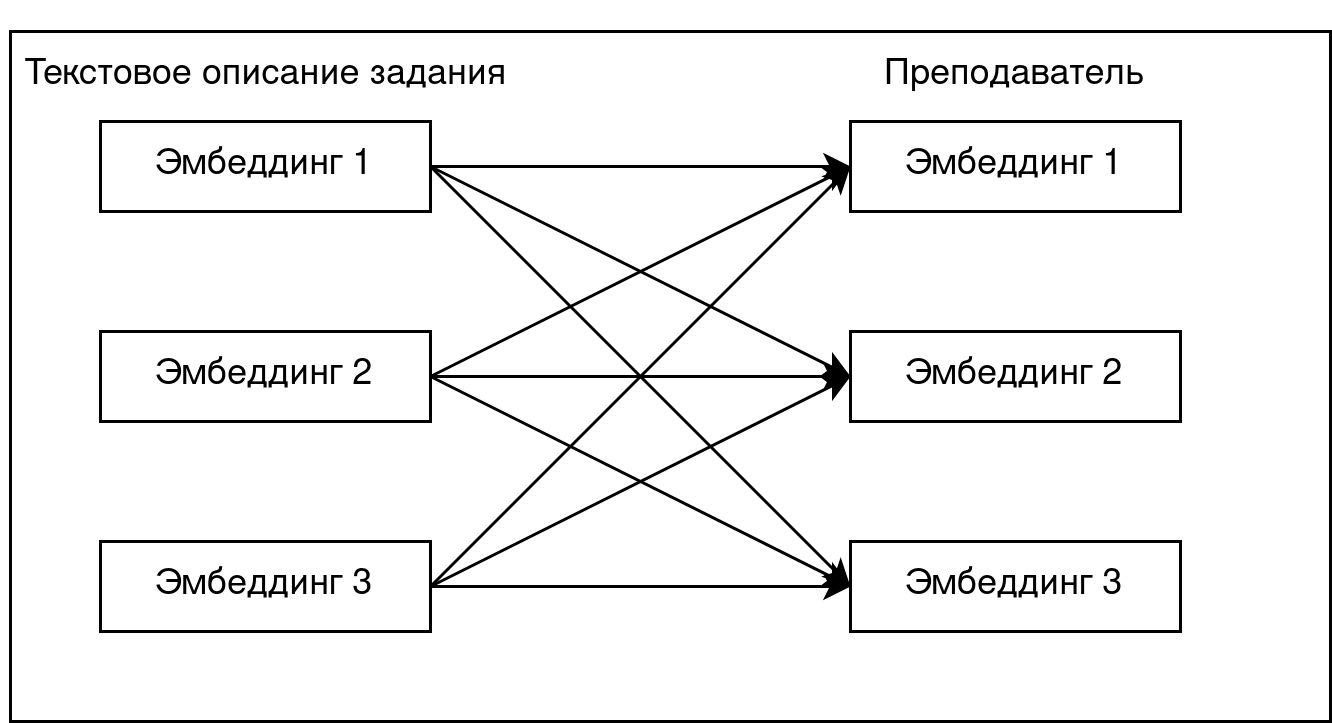
\includegraphics[width=0.6\textwidth]{img/Подбор исполнителя 1}
\end{FIGURE}
\begin{FIGURE}[h]{Поиск минимального с повторами \label{fig:Подбор исполнителя 2}}
	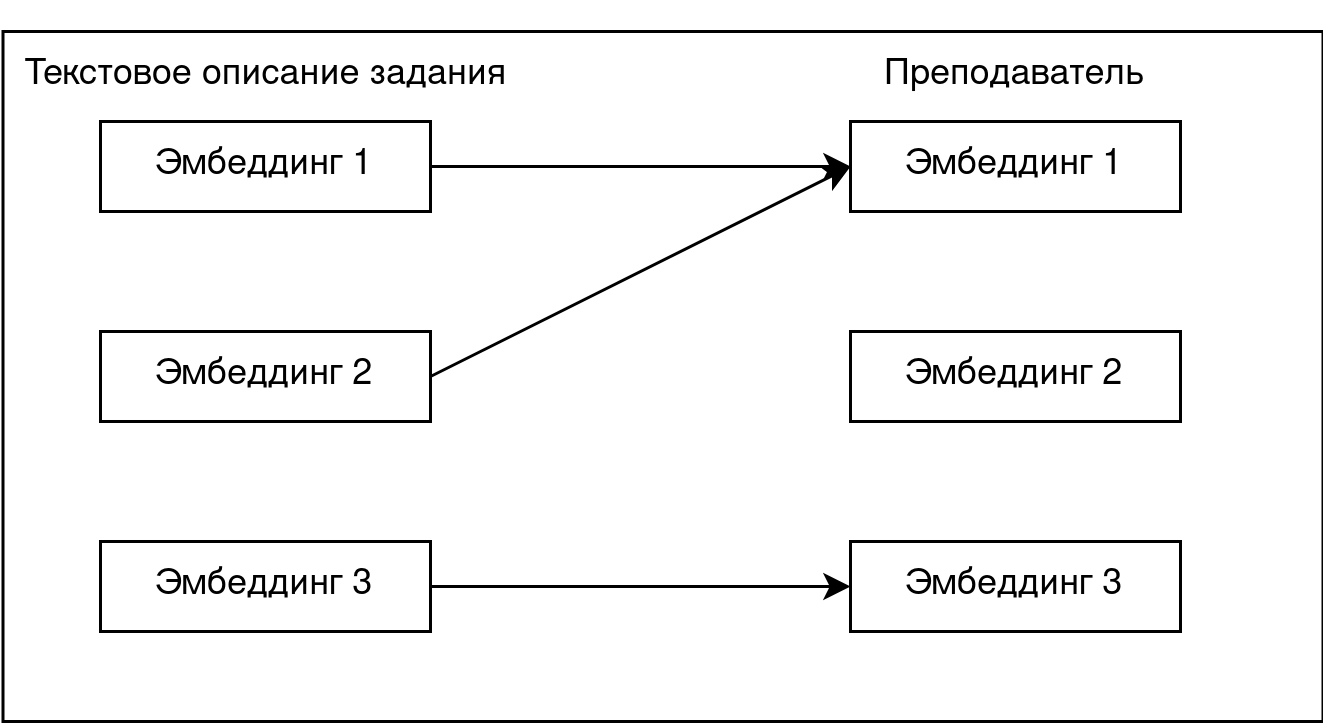
\includegraphics[width=0.6\textwidth]{img/Подбор исполнителя 2}
\end{FIGURE}
\begin{FIGURE}[h]{Поиск минимального без повторов \label{fig:Подбор исполнителя 3}}
	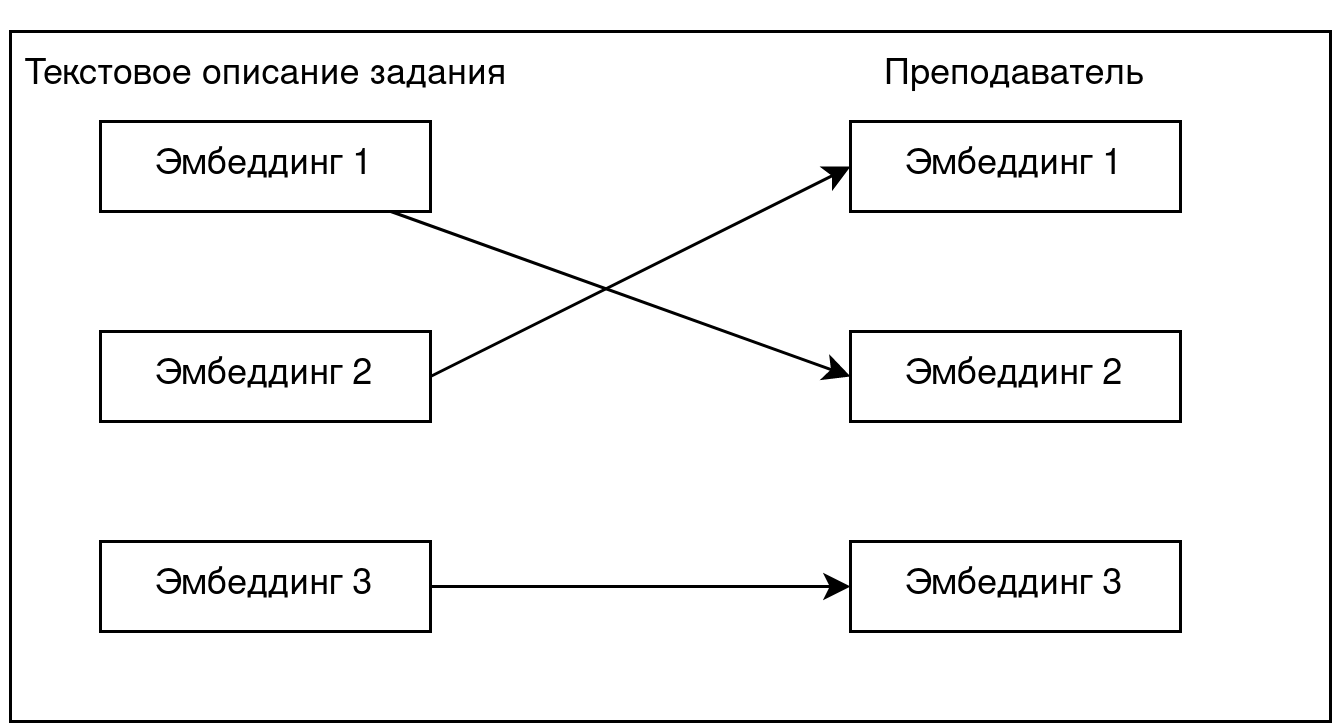
\includegraphics[width=0.6\textwidth]{img/Подбор исполнителя 3}
\end{FIGURE}
\begin{FIGURE}[h]{Усреднение эмбеддингов \label{fig:Подбор исполнителя 4}}
	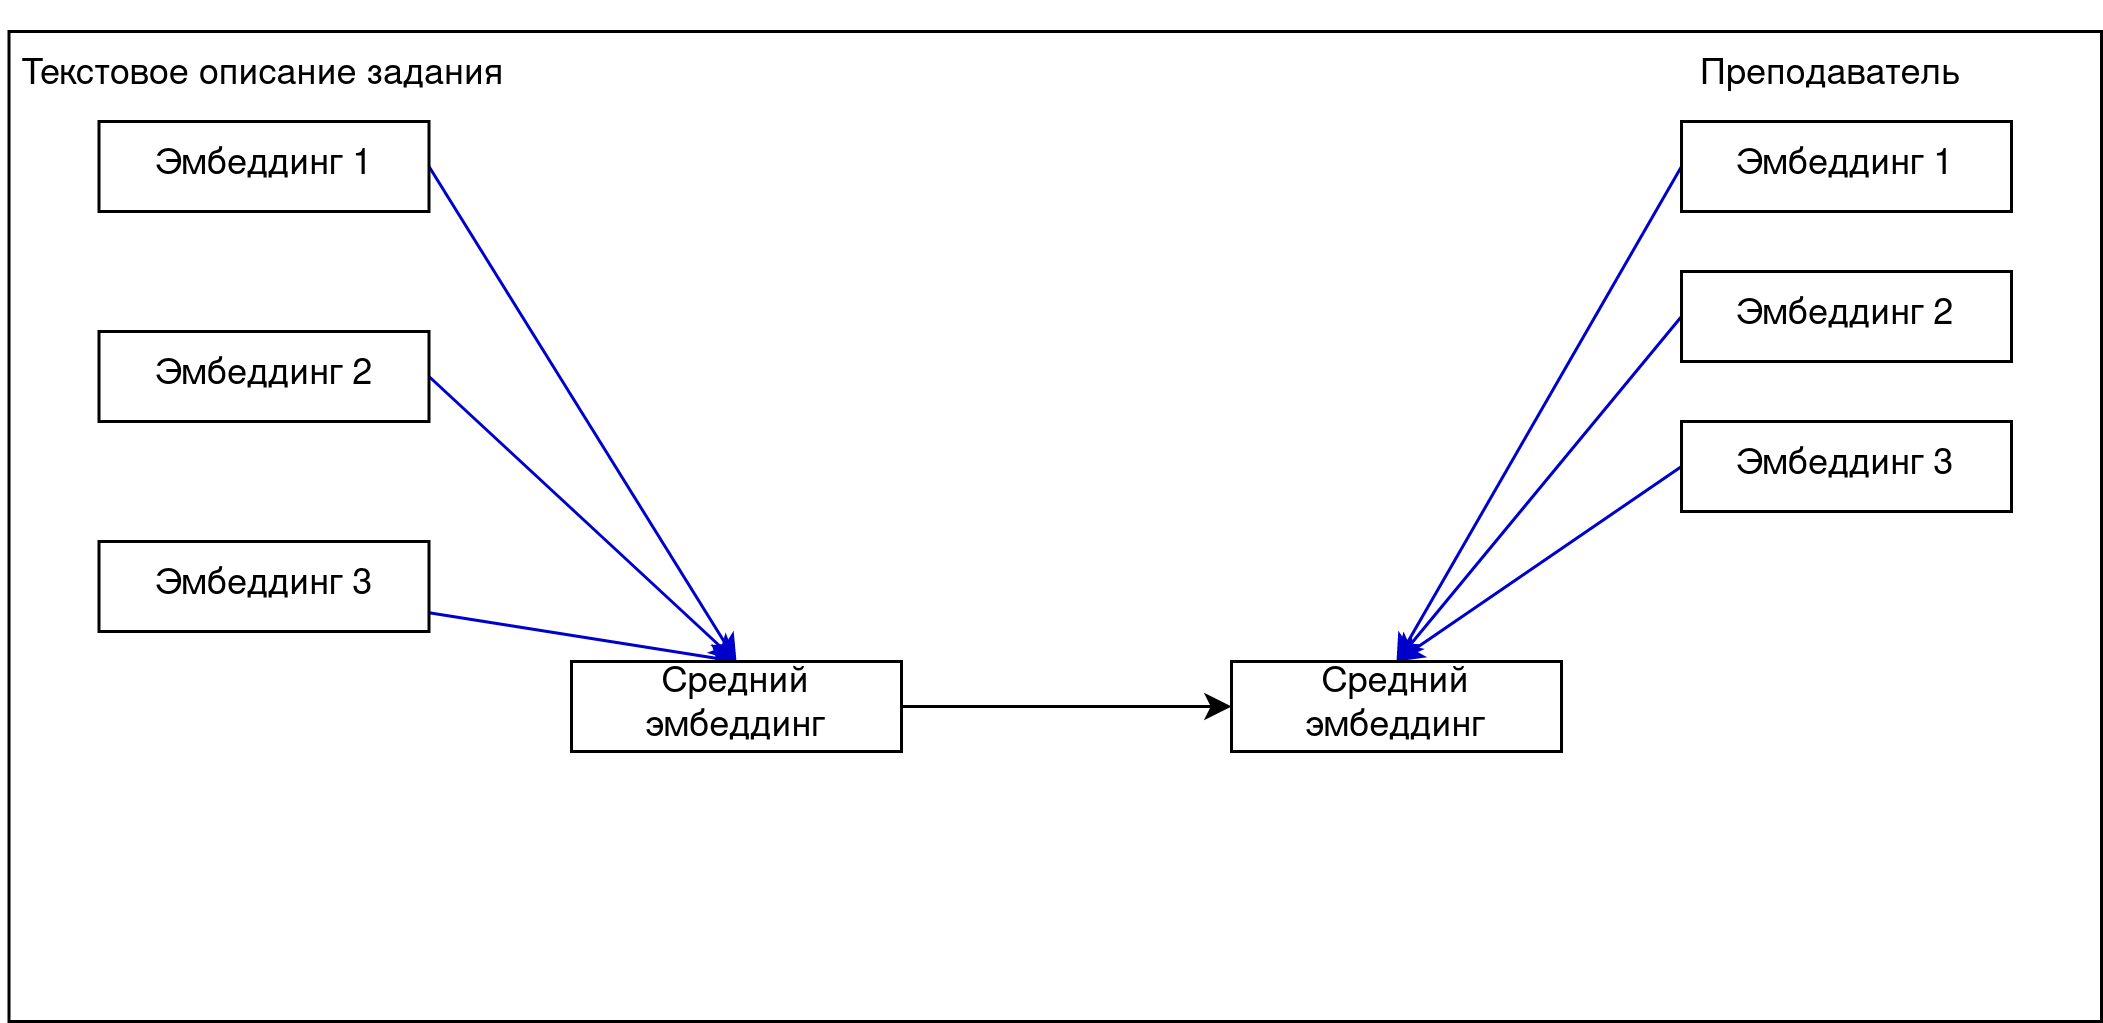
\includegraphics[width=0.6\textwidth]{img/Подбор исполнителя 4}
\end{FIGURE}
\end{document}
